Since the appearance of the first digital computers in 1940s, Monte Carlo (MC) sampling remains one of the most well-known and widely used methods for the analysis of stochastic systems.
The reason for this popularity lies in the ease of implementation, in the independence of the stochastic dimensionality of the considered problems, and in the fact that the quantities estimated using MC simulations asymptotically approach the true values (the laws of large numbers \cite{durrett2010}).
The crucial problem with MC sampling, however, is the low rate of convergence: the error decreases at the order of $\nsamples^{-1/2}$ where $\nsamples$ is the number of samples \cite{xiu2010, maitre2010}.
This means that, in order to get an additional decimal point of accuracy, one has to obtain hundred times more samples.
Each such sample implies a complete realization of the whole system, which renders MC-based methods slow and often infeasible since the number of needed simulations can be extremely large \cite{diaz-emparanza2002}.

In order to overcome the limitations of deterministic power-temperature analysis (PTA) and, at the same time, to completely eliminate or, at least, mitigate the costs associated with MC sampling, a number of alternative stochastic PTA techniques have been recently introduced.
Due to the fact that the leakage component of the power dissipation is influenced by process variation the most \cite{chandrakasan2001, srivastava2010, juan2011, juan2012}, the techniques discussed below primarily focus on the variability of leakage.

A solely power-targeted but temperature-aware solution is proposed in \cite{chandra2010} wherein the driving force of the analysis is MC sampling with partially precomputed data.
A learning-based approach is presented in \cite{juan2011} to estimate the maximal temperature under the steady-state condition.
Temperature-related issues originating from process variation are also considered in \cite{juan2012} where a statistical model of the steady-state temperature based on Gaussian distributions is derived.
In \cite{shen2009}, the theory of polynomial chaos (PC) expansions \cite{xiu2010, maitre2010, ghanem1991, eldred2008} together with principal component analysis (PCA) are employed to estimate the full-chip leakage power.
A generalization of PCA known as the Karhunen-Lo\`{e}ve (KL) decomposition (refer to the same literature as for PC expansions) is used in \cite{bhardwaj2006} for the leakage calculation.
An analysis of the voltage response of power grids is carried out in \cite{ghanta2006} where the PC and KL methods are jointly utilized.

\begin{figure}[br]
  \vspace{-1.0em}
  \centering
  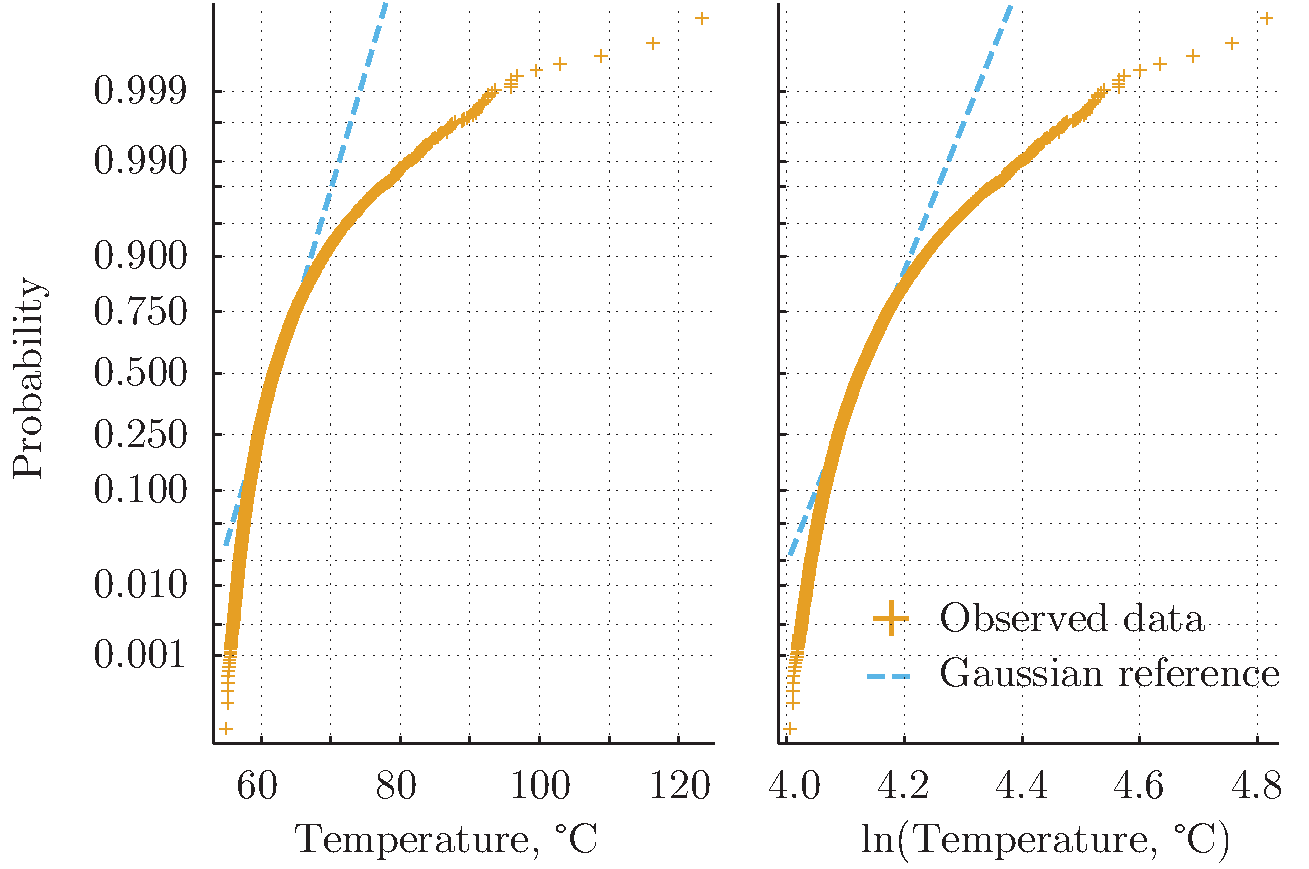
\includegraphics[width=1.0\linewidth]{include/assets/normal-plots.pdf}
  \vspace{-1.5em}
  \caption{Normal probability plots before (on the left) and after (on the right) of the log transformation.}
  \flabel{normal-plots}
\end{figure}

The last three of the aforementioned techniques, \ie, \cite{shen2009, bhardwaj2006, ghanta2006}, are temperature-unaware solutions to power modeling under process variation.
The rest are temperature-related approaches, but none of them attempts to perform stochastic transient PTA and to compute the evolving-in-time probability distribution of temperature.
However, such transient curves are of practical importance.
First of all, certain procedures cannot be undertaken without the knowledge of the time-dependent temperature variations, \eg, reliability optimization based on the thermal-cycling fatigue \cite{ukhov2012}.
Secondly, the constant steady-state temperature assumption, considered, \eg, in \cite{juan2011, juan2012}, can rarely be justified since power profiles are not invariant in reality.
In addition, one can frequently encounter the assumption that power and/or temperature follow \apriori\ known probability distributions, for instance, Gaussian and log-normal distributions are popular choices as in \cite{srivastava2010, juan2012, bhardwaj2006}.
However, this assumption often fails in practice (also noted in \cite{juan2012} regarding the normality of the leakage power) due to: (a) the strict nonlinearities between the process-related parameters, power, and temperature; (b) the nonlinear interdependency of temperature and the leakage power \cite{liu2007}.
To illustrate this, we simulated the example given in \sref{introduction} $10^4$ times assuming the widespread Gaussian model for the variability of the effective channel length; the rest of the experimental setup was configured as it will be described in \sref{illustrative-example} and \sref{experimental-results}.
Then we applied the Jarque-Bera test of normality to the collected data (temperature) directly as well as after processing them with the log transformation.
The null hypothesis that the data are from an unspecified Gaussian distribution was firmly rejected in both cases at the significance level of 5\%.
\fref{normal-plots} gives an example of the normal probability plots inherent to the observed data before (on the left) and after (on the right) the log transformation.
It can be seen that the samples, marked with orange crosses, significantly diverge from the straight blue line that represents a pure Gaussian scenario.
Consequently, the observed distributions of temperature are neither Gaussian nor log-normal, which can also be seen in \fref{experimental-results-pdf} described in the experimental results, \sref{experimental-results}.

To conclude, the published stochastic PTA techniques for electronic system design are restricted in use due to one or several of the following traits: based on MC simulations (potentially slow) \cite{chandra2010}, limited to power analysis \cite{chandra2010, shen2009, bhardwaj2006, ghanta2006}, limited to the assumption of the constant steady-state temperature \cite{juan2011, juan2012}, exclusive focus on the maximal temperature \cite{juan2011}, \apriori\ chosen distributions of power and temperature \cite{srivastava2010, juan2012, bhardwaj2006}.
Thus, there is a lack of flexible stochastic PTA techniques, which we aim to fill in.
